\documentclass[11pt]{amsart}
\usepackage{geometry}                % See geometry.pdf to learn the layout options. There are lots.
\geometry{letterpaper}                   % ... or a4paper or a5paper or ... 
%\geometry{landscape}                % Activate for for rotated page geometry
%\usepackage[parfill]{parskip}    % Activate to begin paragraphs with an empty line rather than an indent
\usepackage{graphicx}
\usepackage{amssymb}
\usepackage{epstopdf}
\usepackage{bm}
\newcommand*{\B}[1]{\ifmmode\bm{#1}\else\textbf{#1}\fi}

\DeclareGraphicsRule{.tif}{png}{.png}{`convert #1 `dirname #1`/`basename #1 .tif`.png}

\usepackage{tikz}
\usetikzlibrary{bayesnet}

\title{Brief Article}
\author{The Author}
%\date{}                                           % Activate to display a given date or no date

\begin{document}
\maketitle
%\section{}
%\subsection{}
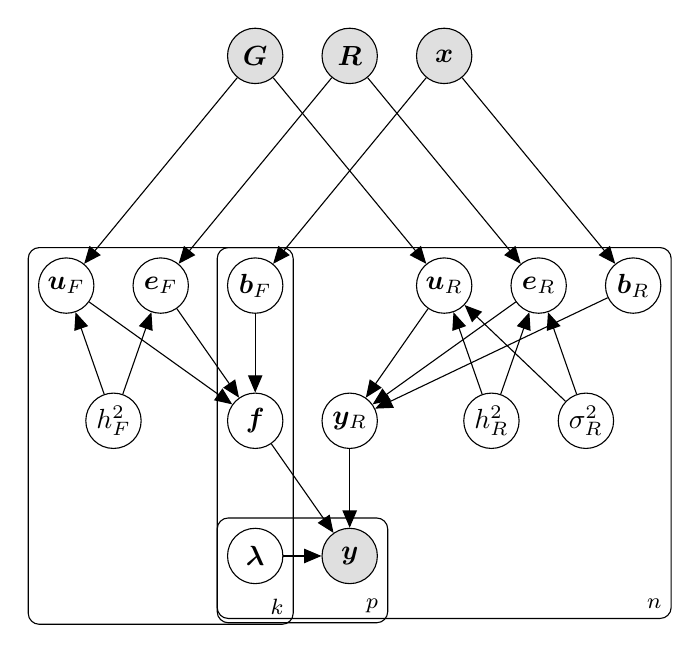
\begin{tikzpicture}

  % Define nodes
  \node[obs]                               				(y) {$\B{y}$};
  \node[latent, xshift=-1.2cm]  (lambda) {$\B{\lambda}$};
  \node[latent, above=of y] 	     			(y_r) {$\B{y}_R$};
  \node[latent, above=of y, xshift=-1.2cm] 		(f) {$\B{f}$};
  \node[latent, above=of f, xshift=-2.4cm]  		(u_f) {$\B{u}_F$};
  \node[latent, above=of f, xshift=-1.2cm]  		(e_f) {$\B{e}_F$};
  \node[latent, above=of f, xshift=0cm]  		(b_f) {$\B{b}_F$};
  \node[latent, above=of y_r, xshift=1.2cm]  	(u_r) {$\B{u}_R$};
  \node[latent, above=of y_r, xshift=2.4cm]  	(e_r) {$\B{e}_R$};
  \node[latent, above=of y_r, xshift=3.6cm]  	(b_r) {$\B{b}_R$};
  \node[latent, below=of u_f, xshift=0.6cm]		(h2_f) {$h^2_F$};
  \node[latent, below=of u_r, xshift=0.6cm]		(h2_r) {$h^2_R$};
  \node[latent, below=of u_r, xshift=1.8cm]		(s2_r) {$\sigma^2_R$};
  \node[obs,above=of b_f, yshift = 1.2cm,xshift=0cm]                (G) {$\B{G}$};
  \node[obs,above=of b_f, yshift = 1.2cm, xshift=1.2cm]             (R) {$\B{R}$};
  \node[obs,above=of b_f, yshift = 1.2cm, xshift=2.4cm]        	(x) {$\B{x}$};         

  
  
  
%  \node[obs]                               (y) {$\B{y}$};
%  \node[latent,xshift=3.6cm]                               (y_r) {$\B{y}_R$};
%  \node[latent, above=of y, xshift=1.2cm] (f) {$\B{f}$};
%  \node[latent, above=of y, xshift=-1.2cm]  (lambda) {$\B{\lambda}$};
%  \node[latent, above=of f, xshift=-2.4cm]  (u_f) {$\B{u}_F$};
%  \node[latent, above=of f, xshift=-1.2cm]  (e_f) {$\B{e}_F$};
%  \node[latent, above=of f, xshift=-0.0cm]  (b_f) {$\B{b}_F$};
%  \node[latent, above=of y, xshift=2.4cm]  (u_r) {$\B{u}_R$};
%  \node[latent, above=of y, xshift=3.6cm]  (e_r) {$\B{e}_R$};
%  \node[latent, above=of y, xshift=4.8cm]  (b_r) {$\B{b}_R$};
%  \node[obs,above=of b_f]                               (R) {$\B{R}$};
%  \node[obs,above=of b_f, xshift=-1.2cm]                               (G) {$\B{G}$};
%  \node[obs,above=of b_f,, xshift=1.2cm]        (x) {$\B{x}$};         

  % Connect the nodes
  \edge {f,lambda,y_r} {y} ; 
  \edge {u_f,e_f,b_f} {f} ; 
  \edge {u_r,e_r,b_r} {y_r} ; 
  \edge {G} {u_f,u_r} ; 
  \edge {R} {e_f,e_r} ; 
  \edge {x} {b_f,b_r} ; 
  \edge {h2_f} {u_f,e_f} ; 
  \edge {h2_r} {u_r,e_r} ; 
  \edge {s2_r} {u_r,e_r} ; 

  % Plates
  \plate{fl}{(f)(lambda)(u_f)(e_f)(b_f)(h2_f)} {$k$} ;
  \plate {yf} {(y)(f)(u_r)(e_r)(b_r)(y_r)(h2_r)(s2_r)} {$n$} ;
  \plate {yp} {(y)(lambda)} {$p$} ;
%  \plate {} {(w)(y)(yx.north west)(yx.south west)} {$M$} ;

\end{tikzpicture}



\end{document}  